% !TEX program = pdflatex
% IEEE conference draft; no venue-specific page limit has been selected.
% The original manuscript is preserved as paper-crewai-original.tex.
% DeepSeek results are interim. The completed Gemma study is historical.
\documentclass[conference]{IEEEtran}
\usepackage[T1]{fontenc}
\usepackage{cite}
\usepackage{amsmath,amssymb}
\usepackage{graphicx}
\usepackage{booktabs}
\usepackage{array}
\usepackage{url}
\usepackage{xcolor}
\usepackage{tikz}
\usetikzlibrary{arrows.meta,positioning,calc}
\graphicspath{{paper-figures/}}
\newcommand{\NEI}{\textsc{nei}}
\newcommand{\CI}{\textsc{ci}}
\newcommand{\modelname}{\texttt{gemma4:31b-cloud}}
\newcommand{\jevname}{\texttt{jev-1.13.0}}
\newcommand{\pct}{\%}

\newcommand{\DeepSeekRows}{%
Selected 50 & Baseline & 24/50 & 0 & 6/24 & 1/0 \\
Selected 50 & Candidate & 23/50 & 15 & 3/23 & 0/0 \\
Other 450 & Baseline & 0/450 & 0 & -- & 0/0 \\
Other 450 & Candidate & 0/450 & 0 & -- & 0/0 \\
Pooled 500 & Baseline & 24/500 & 0 & 6/24 & 1/0 \\
Pooled 500 & Candidate & 23/500 & 15 & 3/23 & 0/0 \\
}

\begin{document}
\title{Evidence Gates and Failure-Inclusive Evaluation for Claim Verification with KajiAI}

% Set authors, affiliations and any anonymity requirements after selecting a venue.
\author{\IEEEauthorblockN{Anonymous review draft}}
\maketitle

\begin{abstract}
KajiAI is a LangGraph workflow that separates proposed factual labels from evidence acceptance and retains retrieved text versions for audit. We froze a comparison of the current workflow and an evidence-adjudicated candidate on 500 AVeriTeC development claims with DeepSeek and a fixed Jev verifier. This interim analysis accounts for 47 of 1,000 scheduled cells, all carried forward from a resource pilot. The baseline proposed 6 correct labels in 24 cells and accepted one. The candidate proposed 3 correct labels in 23 cells, had 15 execution failures and accepted zero. Across 23 terminal pairs, the candidate-minus-baseline proposal agreement difference was $-8.7$ percentage points (95\pct\ paired bootstrap interval $-30.4$ to $+13.0$). The other 450 claims remain untouched in this comparison. The separate historical Gemma study measured a 13.6-point gain over a model-only control, and a controlled stopping challenge forfeited two correct acceptances when it skipped reassessment. These studies use different configurations and answer different questions. Pilot-based model selection, live retrieval, incomplete coverage and outstanding human citation adjudication limit inference.
\end{abstract}

\begin{IEEEkeywords}
automated fact-checking, retrieval-augmented generation, LangGraph, citation provenance, selective prediction, AVeriTeC
\end{IEEEkeywords}

\section{Introduction}
Automated fact-checking requires more than assigning a plausibly correct label. A system should identify evidence, connect that evidence to the claim, disclose uncertainty and preserve enough provenance for inspection. FEVER established an evidence-oriented task using claims derived from Wikipedia \cite{fever}. AVeriTeC extends this setting to real-world claims and web evidence \cite{averitec}. Its shared-task score combines verdict correctness with evidence quality \cite{sharedtask}, emphasizing that label agreement alone is an incomplete account of verification.

Retrieval-augmented generation provides external information to a language model \cite{rag}, but retrieved documents, citations and repeated reasoning do not themselves guarantee an evidence-supported verdict. Citation evaluation distinguishes answer correctness from citation quality \cite{alce}. This distinction motivates an architecture in which prediction and acceptance are observable, separate decisions.

We present KajiAI, an auditable workflow implemented with LangGraph. A model proposes a factual label and an evidence assessment. A gate checks retrieved citations, exact quotations, assertion coverage, source-host diversity and domain requirements, followed by automated semantic citation review. Failed checks preserve the prediction while withholding an accepted verdict. Unresolved gaps can trigger further research, subject to limits on rounds, searches, page fetches, elapsed time and reported tokens.

The frozen DeepSeek comparison asks how an evidence-adjudicated candidate changes proposal agreement, acceptance coverage, execution failures and resource use relative to the standard workflow. We report the exposed pilot stratum separately from the other 450 cases. Historical studies give two different comparisons: Gemma with and without the workflow, and three cloud models under scripted fixed-evidence stopping.

The evaluation treats operational failure as a result. It preserves each started cell and the service reservations associated with it. Source versions and saved assessments support inspection of disagreements among label agreement, evidence checks and resource use.

\section{Related Work}
\subsection{Evidence-Based Fact-Checking}
FEVER pairs supported and refuted claims with annotated evidence sentences \cite{fever}. AVeriTeC uses real-world claims, question--answer evidence and textual justifications from web sources \cite{averitec}. The AVeriTeC shared task evaluates evidence retrieval and veracity prediction jointly \cite{sharedtask}. We use its development labels for a local four-class study; our scores are not official AVeriTeC scores and cannot be directly compared with shared-task rankings.

The 2025 AVeriTeC shared task instead specifies open-weight models, a precompiled evidence store, a single-GPU resource constraint and a one-minute processing limit \cite{sharedtask2025}. Our cloud-assisted, contemporary-web protocol does not reproduce those conditions.

\subsection{Retrieval and Citation Evaluation}
RAG combines parametric generation with external document memory \cite{rag}; Self-RAG learns retrieval and critique through reflection tokens \cite{selfrag}. KajiAI instead uses structured assessments, query templates and explicit routing rules, allowing inspection of query generation and stopping behavior.

FIRE integrates retrieval and verification iteratively, choosing a final judgment or another search query using confidence \cite{fire}. EMULATE distributes search-result ranking and webpage-content assessment across agents \cite{emulate}. Iterative research and role separation therefore precede KajiAI. Our empirical focus is preserving source versions, separating provisional prediction from rule-based acceptance, and measuring changes across frozen trajectories.

ALCE evaluates generated answers along fluency, correctness and citation quality dimensions \cite{alce}. Our literal-quote check addresses a narrower property: whether a quoted string occurs in stored text for its cited URL. A separate model reviews whether that quotation supports its attached finding. Neither mechanism independently establishes the truth of the overall verdict.

\subsection{Selective Prediction}
Selective classification trades coverage for accuracy through rejection \cite{selective}. KajiAI selects outputs through evidence requirements; its confidence categories and citation-review scores lack independent calibration, so the reported coverage and conditional label accuracy carry no statistical risk guarantee.

\section{System Design}
\subsection{Stateful Graph and Execution}
LangGraph supports stateful workflows combining deterministic operations and model calls \cite{langgraph}. Eight nodes execute KajiAI's process in Fig.~\ref{fig:architecture}. The shared state includes the original claim, optional reference date, domain, assertions, retrieval ledger, research history, proposed assessment, evidence gaps, budgets and stop reason. Individual claims follow a sequential graph. The frozen DeepSeek comparison uses one worker. The historical Gemma runner used up to three.

\begin{figure}[t]
\centering
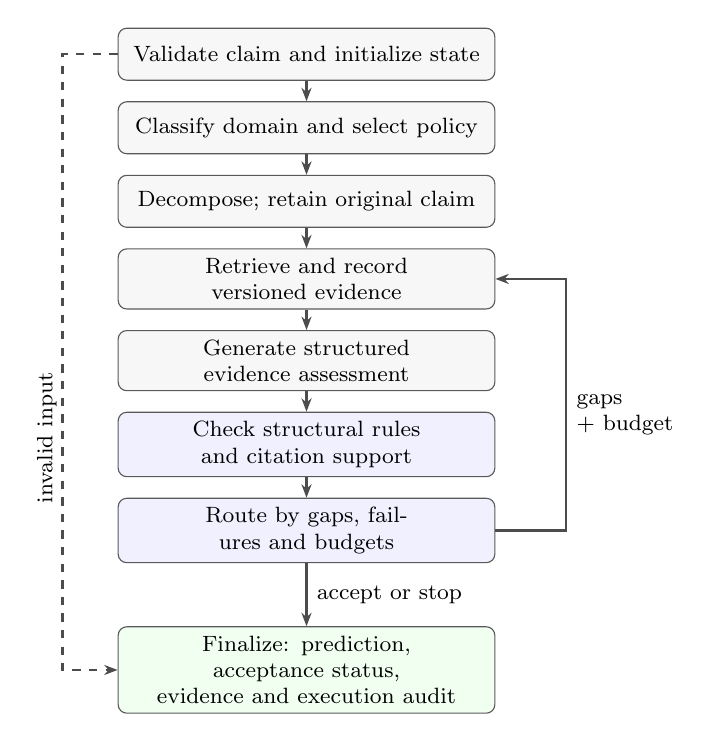
\begin{tikzpicture}[
  node distance=2.6mm,
  flowblock/.style={draw=black!65, rounded corners=1.1mm,
    fill=black!3, align=center, text width=4.55cm,
    minimum height=6.6mm, font=\footnotesize},
  flowgate/.style={flowblock, fill=blue!6},
  flowarrow/.style={-{Stealth[length=1.7mm]}, thick, draw=black!70}
]
\node[flowblock] (validate) {Validate claim and initialize state};
\node[flowblock, below=of validate] (classify) {Classify domain and select policy};
\node[flowblock, below=of classify] (decompose) {Decompose; retain original claim};
\node[flowblock, below=of decompose] (retrieve) {Retrieve and record versioned evidence};
\node[flowblock, below=of retrieve] (analyze) {Generate structured evidence assessment};
\node[flowgate, below=of analyze] (check) {Check structural rules and citation support};
\node[flowgate, below=of check] (route) {Route by gaps, failures and budgets};
\node[flowblock, below=8mm of route, fill=green!6] (finalize)
  {Finalize: prediction, acceptance status,\\evidence and execution audit};
\foreach \from/\to in {validate/classify,classify/decompose,
  decompose/retrieve,retrieve/analyze,analyze/check,check/route}
  \draw[flowarrow] (\from) -- (\to);
\draw[flowarrow] (route) -- node[right, font=\footnotesize] {accept or stop} (finalize);
\draw[flowarrow] (route.east) -- ++(9mm,0)
  |- node[pos=0.23, right, font=\footnotesize, align=left]
  {gaps\\+ budget} (retrieve.east);
\draw[flowarrow, dashed] (validate.west) -- ++(-7mm,0) |-
  node[pos=0.25, left, xshift=-2mm, font=\footnotesize, rotate=90] {invalid input}
  (finalize.west);
\end{tikzpicture}
\caption{Explicit stateful workflow. Remaining gaps can trigger retrieval; failures, stagnation and budgets stop research. Finalization independently rechecks acceptance conditions.}
\label{fig:architecture}
\end{figure}

The DeepSeek comparison uses the exact Ollama tag \texttt{deepseek-v4.1-flash:cloud} through a loopback service and checks the returned model ID. TinyFish Search and Fetch and TypeSafe Jev supply the other network services. Within one attempt the retriever reuses fetched pages. Each arm starts a fresh workflow state. The coordinator saves checkpoints at attempt boundaries. The graph itself has no persistent checkpoint store.

Jev, accessed through the TypeSafe SDK, supplies the workflow's domain, search-ranking, source-review and citation-support judgments. Domain classification uses Jev when its confidence is at least 0.6, with an Ollama classifier and then keyword scoring as fallbacks. The profiles are general, scientific, political and health/medical. The baseline uses a deterministic conjunction heuristic limited to six fragments. Fragments act as coverage obligations within the assessment. The candidate adds neutral research questions as guidance while retaining the heuristic coverage obligations and the original claim.

\subsection{Query Construction and Retrieval}
At round $t$, the standard workflow constructs an ordered list from (i) follow-up queries proposed in the previous assessment, (ii) the claim plus \lq\lq evidence,'' (iii) the claim plus \lq\lq counterevidence,'' (iv) each assertion plus \lq\lq evidence,'' and (v) each assertion plus \lq\lq original source fact check.'' It trims and deduplicates strings, excludes previously used queries and selects the first two remaining candidates when the budget permits.

The standard workflow combines model suggestions with hardcoded templates. The candidate places verification questions after prior follow-up queries, prepends primary-source queries when a provenance gap is active, and can move an eligible source-reference query into the second slot. No learned optimizer chooses the best query. Jev ranks returned URLs for fetching, a separate decision from choosing a query. TinyFish supplies up to five results per search and up to two full-page fetch attempts per search. Failed fetches leave available snippets in the ledger.

A source record stores the URL, query, provider, retrieval time, snippet or page text, content hash and review scores. Full-page text is preferred to a snippet for the same URL, truncated to 20,000 characters and hashed after truncation. The canonical record used in an assessment is retained by URL and hash, permitting replay against the same text version. Jev source review estimates relevance, evidence value, counterevidence value and injection risk. Reviewed records with injection score at least 0.9, or all three relevance/evidence scores below 0.1, are excluded from usable evidence. Unreviewed records retain permissive defaults; this filter is not a demonstrated injection defense.

\subsection{Prediction and Acceptance}
The analyzer returns a structured assessment containing a verdict, confidence category, findings, cited URLs, quotations, assertion resolutions, contradictions, gaps and next queries. It also reports source independence, counterevidence search and, where required, peer-reviewed support. These model-reported flags are policy inputs rather than independently verified facts.

Let $\hat y_i$ be the proposed label for claim $i$, and $G_{s,i}$ and $G_{m,i}$ its structural and semantic gap sets. Acceptance is
\begin{equation}
a_i=\mathbf{1}\{G_{s,i}=\varnothing,\ G_{m,i}=\varnothing,\ F_i=0\},
\label{eq:acceptance}
\end{equation}
where $F_i$ indicates execution failure. The accepted output is
\begin{equation}
\tilde y_i =
\begin{cases}
\hat y_i, & a_i=1,\\
\bot, & a_i=0,
\end{cases}
\label{eq:selective}
\end{equation}
where $\bot$ is operational abstention, not the factual \NEI\ class.

Structural acceptance requires a decisive verdict and High confidence; nonempty retrieved citations for every finding; literal quotations in canonical source text; complete assertion coverage; at least two cited hosts; no flagged duplicate lineage among cited sources; and no unresolved gaps or contradictions. A token-set Jaccard threshold of 0.85 flags substantially similar source text. Counterevidence and independence flags must be positive. Scientific claims require HTTPS citations; health/medical claims require the peer-review flag. A conflicting verdict additionally requires supporting and refuting findings. Established disagreement belongs in those findings and the summary; the contradictions field instead records unresolved objections to the proposed verdict. Distinct hosts, text dissimilarity and model flags do not prove actual independence.

For each eligible finding--URL--quotation triple, Jev reviews the quotation and up to 1,200 surrounding characters on each side. Semantic acceptance requires a \lq\lq supports'' relation with confidence at least 0.8 for every citation. Missing or failed citation checks block acceptance. Review identity includes finding, URL, quotation and content hash; finalization repeats structural checks and confirms review coverage. This tests quotation support for an attached finding, not the entire inferential chain from documents to verdict.

\subsection{Bounded Research and Auditability}
When gaps remain, routing allows further research if execution has not failed and resource and stagnation limits permit it. Two consecutive rounds with no new ledger records trigger a stagnation stop. A new record can be a changed snippet for an already fetched URL, so ledger growth is not equivalent to new usable evidence.

Each round retains its raw assessment, exact usable source versions, gaps, budget snapshot, elapsed time and stop decision. Reported token usage is aggregated, with a completeness flag when accounting is unavailable. Time and token limits govern scheduling; an in-flight request can finish after the soft deadline or exceed the reported-token threshold. Missing usage prevents a guaranteed spend cap. The report preserves proposed and accepted verdicts separately and distinguishes insufficient evidence from execution errors.

\subsection{Evidence-Adjudicated Candidate}
The candidate first selects literal passages by ID and proposes a factual class. It evaluates passage stance and checks source paths separately, using source-bound anchors from a predecision review. The origin-review head adjudicates the acceptance materiality of each lead. A material or unresolved class-undermining issue blocks acceptance. The compiler resolves selected IDs to their original retained text and rejects invalid bindings. An additional independent-provenance review is required before acceptance. Source references found during research can supply a follow-up query within the existing round budget.

The executable path is the archived \path{flash_study.py} worker and \path{graph.py} runtime. The candidate uses \path{evidence_adjudicated.py}, \path{source_paths.py} and \path{passage_decision.py}. The current command-line defaults in \path{config/default.yaml} use standard assessment and Gemma. Query-exhaustion stopping is opt-in and disabled in both DeepSeek arms. The current tree's unfinished \path{semantic_evidence.py} integration is outside the frozen archive. The companion code audit maps these paths to the archived versions and fixture tests.

\section{Evaluation Protocol}
\subsection{Frozen DeepSeek Comparison}
The shared manifest contains 500 distinct AVeriTeC development claims. We preserved the earlier seeded 50-case pilot order and each case's relative DeepSeek arm order. The other 450 follow manifest order and alternate the first arm. Both arms receive only claim text and date. The analysis joins labels offline. The retained early pilot records were bound to the frozen source, configuration and raw journal hashes. A started cell remains in the ledger even if its workflow fails.

\begin{table}[t]
\caption{Frozen settings for the two DeepSeek arms}
\label{tab:deepseek-settings}
\centering
\footnotesize
\begin{tabular}{@{}p{.31\columnwidth}p{.61\columnwidth}@{}}
\toprule
Setting & Value\\
\midrule
Shared & DeepSeek V4.1 Flash cloud at temperature zero; Jev 1.13; three rounds; one worker; 270 s graph budget and 300 s worker limit\\
Standard arm & Standard assessment; 4,096 requested output tokens; original reasoning behavior\\
Candidate arm & Evidence adjudication, bound anchors, separate materiality judgment and provenance review; requests up to 6,144 assessment or 2,048 planning output tokens; reasoning disabled on both request types\\
Transport & Per cell, at most 8 Ollama, 40 Jev, 6 Search and 12 Fetch URLs; zero external retries\\
Retrieval pacing & 27 searches/min and 450/hour; 135 Fetch URLs/min and 900/rolling 24 h\\
\bottomrule
\end{tabular}
\end{table}

Table~\ref{tab:deepseek-settings} lists the combined intervention. Generic classification can retain original reasoning behavior in the candidate and uses its 6,144-token ceiling. The archived native GLM trial of the candidate failed its source-fidelity check on an unsupported scope and materiality concern. The native check closed before the planned eight-case development and twelve-case confirmation screens were released. The DeepSeek comparison waived qualification for entry while retaining the acceptance checks. Early outcomes influenced the choice of DeepSeek. On 23 paired cases shared with the pilot's GLM arm, baseline proposals agreed with gold on 5 cases for DeepSeek and 3 for GLM, and candidate proposals agreed on 3 and 2. Execution failures were 0 and 2 for the baseline and 15 and 18 for the candidate, in the same model order. The earlier Gemma run used different conditions.

We count execution failures as disagreement and withhold acceptance on failures. We report the proportions over observed terminal cells, plus candidate-minus-baseline differences from terminal pairs with a case-level percentile bootstrap. Correct acceptance refers to label agreement after the automated gate. Independent human evidence annotation remains outstanding. The official AVeriTeC evidence score is outside this protocol.

\subsection{Historical Gemma Dataset and Conditions}
The completed study assesses all 500 AVeriTeC development claims in two conditions. The split contains 122 Supported, 305 Refuted, 35 Not Enough Evidence and 38 Conflicting Evidence/Cherrypicking labels. Only claim text and claim date are supplied as dataset inputs to inference. Gold labels, justifications and annotated evidence are reserved for scoring and post hoc audit. Both conditions use the same model, temperature and structured-output adapter.

The \emph{model-only control} produces one verdict from existing model knowledge without search, domain routing or an evidence gate. The \emph{full workflow} applies the architecture above. Their comparison measures the combined workflow, including its different prompt and evidence context; it does not isolate retrieval, Jev or LangGraph individually. The \emph{first-round analysis} truncates saved full-workflow trajectories rather than constituting a separately executed system.

\begin{table}[t]
\caption{Frozen Evaluation Configuration}
\label{tab:protocol}
\centering
\footnotesize
\begin{tabular}{@{}p{0.38\columnwidth}p{0.55\columnwidth}@{}}
\toprule
Setting & Value\\
\midrule
Main model / temperature & \modelname\ / 0\\
Review model / threshold & \jevname\ / 0.8\\
Research limits per claim & 3 rounds; 300 s soft deadline\\
Search / fetch ceilings & 20 logical searches; 20 fetches\\
Budgeted reported tokens & 250,000 aggregate reported tokens\\
Per-round retrieval & Up to 2 queries; 2 fetches/query\\
Study scheduling & 3 workers; seed 20261009\\
Installed libraries & LangGraph 1.2.11; Pydantic 2.13.5; TypeSafe SDK 0.7.1\\
\bottomrule
\end{tabular}
\end{table}

Table~\ref{tab:protocol} summarizes the protocol. Claim-condition tasks were shuffled with a fixed seed, but contemporary search and cloud-model responses remain externally variable. Source, configuration, package versions, dataset bytes and hashes are archived. Earlier exploratory runs used different source versions and are excluded. Resume checks reject changes to the frozen inference configuration.

The local reproducibility bundle, \texttt{study-20261009-v3}, contains the run manifest, source archive, dataset snapshot, raw JSONL records and per-claim replay results. Source and dataset SHA-256 prefixes are \texttt{624a8d2fa125} and \texttt{499793726b4a}, respectively; the manifest retains their complete hashes. The plotting script reads saved metrics, without issuing additional service calls.

The study retains all 1,000 planned claim-condition attempts, including 8 workflow and 5 control execution failures. A monthly quota limit interrupted execution after 302 workflow and 283 control attempts; seven quota failures remain recorded. Later concurrent-slot timeouts and a local Ollama restart interrupted two pending control requests. Only unattempted tasks were resumed, with the original model, source, dataset and settings; recorded failures were never retried or replaced. Full incident details accompany the reproducibility bundle.

\subsection{Metrics and Uncertainty}
The evaluation schema maps TRUE, FALSE, NOT\_ENOUGH\_EVIDENCE and CONFLICTING to the four dataset labels. Generic MISLEADING predictions are not equated with the conflicting-evidence class. The evidence gate accepts decisive labels only, excluding \NEI\ by design. Accepted \NEI\ recall is therefore zero even when raw predictions are correct.

For $n$ attempted claims and gold labels $y_i$, raw accuracy, coverage and selective accuracy are
\begin{align}
A &= \frac{1}{n}\sum_{i=1}^{n}\mathbf{1}\{\hat y_i=y_i\},\\
C &= \frac{1}{n}\sum_{i=1}^{n}a_i,\\
A_{\mathrm{sel}} &=
\frac{\sum_{i=1}^{n}a_i\mathbf{1}\{\hat y_i=y_i\}}
{\sum_{i=1}^{n}a_i}.
\end{align}
Selective accuracy is undefined when no output is accepted. Macro F1 averages F1 across the four gold classes; abstentions contribute missed predictions without becoming a fifth gold class. End-to-end accepted-label accuracy is $C A_{\mathrm{sel}}$, preventing conditional accuracy from obscuring low coverage.

Fatal errors remain in the denominator. Failure-inclusive scoring treats them as abstentions; raw scoring can preserve an earlier prediction if a later service fails. Raw and failure-inclusive accuracies coincide. We report 95\pct\ Wilson intervals for proportions, a paired accuracy bootstrap with 2,000 claim-level resamples and seed 20261009, and an exact two-sided McNemar test. These intervals treat claims as sampling units; they do not capture correlated topics, shared-source effects, model drift, service availability or web changes.

\subsection{Offline Policy Replay and Citation Audit}
Policy replay applies alternative acceptance rules to the same saved final assessments and source versions. We compare structural-only acceptance with the full gate and semantic thresholds from 0.5 to 0.95. Replay cannot show how changing a gate would alter later retrieval or reasoning. Removing exact-quote requirements also changes eligibility for semantic review, so it is not an isolated semantic ablation.

Citation measurements count finding--URL occurrences in final assessments, including repeated URLs across findings. A blinded human-audit worksheet contains 454 citation rows from 44 accepted and 50 sampled rejected claims; labels and acceptance status are stored separately. Human annotation fields remain blank. Automated Jev judgments are measurements rather than independent human ground truth.

\section{Results}
\subsection{Interim DeepSeek Comparison}
The interim snapshot retains 47 of the 1,000 scheduled cells. The fresh run is checkpointed before its first new cell because the earlier pilot left fewer than the 12 Fetch URL slots reserved for a new cell. The other 450 claims contribute zero terminal cells. Table~\ref{tab:deepseek-results} uses observed cells as denominators for agreement and reports terminal counts against the target. All 24 baseline cells completed. Eight candidate cells completed and 15 failed. Neither arm timed out. Baseline acceptance coverage was 1/24, with one correct acceptance on the unpaired baseline cell. Candidate coverage was 0/23. Across the 23 terminal pairs, baseline and candidate correctly proposed 5 and 3 labels. The paired difference was $-8.7$ percentage points (95\pct\ paired bootstrap interval $-30.4$ to $+13.0$). No correct or incorrect acceptance occurred on the matched pairs.

\begin{table*}[t]
\caption{Interim DeepSeek outcomes. Accepted counts show correct/incorrect labels. Untouched cells contribute to the planned counts only.}
\label{tab:deepseek-results}
\centering
\footnotesize
\begin{tabular}{@{}llrrrr@{}}
\toprule
Stratum & Arm & Terminal/planned & Failed & Correct proposals & Accepted\\
\midrule
\DeepSeekRows
\bottomrule
\end{tabular}
\end{table*}

The reused cells generated 1,536,161 input and 395,590 output tokens on Ollama and 1,496,816 input and 185,349 output tokens on Jev. They reserved 185 searches and 366 Fetch URLs. Worker time including startup was about 70.4 minutes. At peak uncached list rates these tokens imply estimated costs of \$0.936 for Ollama and \$0.063 for Jev. Provider charges and cache or reasoning counts remain unavailable where the response does not report them. The journal separates worker time from quota waits and calendar time. Fresh usage is zero at this checkpoint.

\subsection{Historical Gemma Paired Label Prediction}
Both conditions assess the same 500 claims: 122 Supported, 305 Refuted, 35 \NEI\ and 38 Conflicting labels. Table~\ref{tab:prediction} reports the paired label results, including failed attempts.

\begin{table}[t]
\caption{Prediction Results on All 500 Claims}
\label{tab:prediction}
\centering
\footnotesize
\begin{tabular}{@{}lrrr@{}}
\toprule
Condition & Accuracy (\pct) & 95\pct\ \CI & Macro F1\\
\midrule
Always Refuted & 61.0 & 56.7--65.2 & 0.189\\
Model only & 53.8 & 49.4--58.1 & 0.417\\
First round$^{\dagger}$ & 68.8 & 64.6--72.7 & 0.530\\
Final workflow & 67.4 & 63.2--71.4 & 0.500\\
\bottomrule
\end{tabular}
\par\smallskip
\parbox{\columnwidth}{\footnotesize $^{\dagger}$Saved-trajectory truncation, not a separate live one-round condition. Wilson intervals; local label metrics, not official AVeriTeC evidence scores.}
\end{table}

Full predictions are correct on 337 claims, compared with 269 for the control. The workflow is correct on 117 claims missed by the control, while the control is correct on 49 missed by the workflow; both are correct on 220 and both are wrong on 114. The paired accuracy difference is 13.60 percentage points (bootstrap 95\pct\ \CI: 8.60--18.60); exact McNemar \(p=1.35\times 10^{-7}\).

The majority baseline achieves 61.0\pct\ accuracy because Refuted dominates the split, but its macro F1 is only 0.189. The workflow improves accuracy and macro F1 over the model-only control. It predicts the conflicting class 98 times, compared with 38 gold conflicting labels. Its \NEI\ recall is 17.1\pct, compared with 40.0\pct\ for the control. Improvement is therefore not uniform across classes.

\subsection{Selective Acceptance}
Table~\ref{tab:acceptance} compares acceptance rules on all 500 saved final assessments. Raw prediction accuracy and accepted-label accuracy represent different outcomes.

\begin{table}[t]
\caption{Acceptance Replay on 500 Final Assessments}
\label{tab:acceptance}
\centering
\footnotesize
\begin{tabular}{@{}lrrr@{}}
\toprule
Policy & Accepted & Coverage (\pct) & Correct / accepted\\
\midrule
Structural only & 50 & 10.0 & 45/50 (90.0\pct)\\
Structural + Jev & 44 & 8.8 & 42/44 (95.5\pct)\\
\bottomrule
\end{tabular}
\par\smallskip
\parbox{\columnwidth}{\footnotesize Conditional accuracy 95\pct\ \CI: 78.6--95.7\pct\ for structural-only replay; 84.9--98.7\pct\ for the full gate.}
\end{table}

The full gate withholds 6 outputs accepted by structural-only replay: 3 wrong labels and 3 correct labels. It accepts 35 Refuted and 9 Supported. Its coverage interval is 6.6--11.6\pct, and end-to-end accepted-label accuracy is 8.4\pct. The gate leaves 295 correct predictions and 161 other attempts unaccepted. Its 95.5\pct\ conditional accuracy describes a small selected subset.

The selected gold labels are 33 Refuted, 9 Supported and 2 Conflicting; the 35 Refuted and 9 Supported counts above describe predictions. On these same 44 IDs, the model-only control matches 30 labels (68.2\pct), while the workflow matches 42. This is a descriptive comparison on a workflow-selected subset, not an independent test of the gate's causal benefit. Selecting only High-confidence assessments instead retains 429 claims with 326 matching labels (76.0\pct); these differently selected cohorts do not establish a calibrated risk guarantee.

Both accepted errors, IDs 353 and 404, have gold conflicting-evidence labels but receive Refuted predictions. In ID 353, the saved assessment uses findings about compensation and legal action to adjudicate a claim specifically about unlicensed vaccines. In ID 404, it combines official denials of complete railway privatization and job losses with reporting about employees' future job-security fears. These illustrative records expose a gap between supporting individual findings and resolving the claim's qualifications and temporal scope. They are case inspections rather than completed human citation annotations.

Figure~\ref{fig:threshold} shows descriptive threshold replay. Stricter thresholds reduce coverage, while lower thresholds can admit additional outputs. Selecting a threshold from this development analysis would require separate validation.

\begin{figure}[t]
\centering
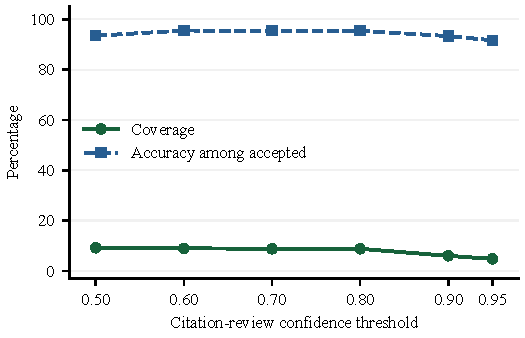
\includegraphics[width=\columnwidth]{acceptance-thresholds.pdf}
\caption{Semantic-threshold replay on 500 final assessments, holding evidence and structural rules fixed. Accepted counts at thresholds 0.50, 0.60, 0.70, 0.80, 0.90 and 0.95 are 46, 45, 44, 44, 30 and 24. The curve does not establish an optimal threshold.}
\label{fig:threshold}
\end{figure}

\subsection{Changes Across Saved Research Rounds}
First-round accuracy is 68.8\pct, compared with 67.4\pct\ for final predictions. Additional rounds change 62 predictions: 18 wrong-to-correct, 25 correct-to-wrong and 19 between incorrect labels. The final-minus-first difference is \(-1.40\) percentage points (bootstrap 95\pct\ \CI: \(-4.00\) to \(1.20\)). Excluding 8 fatal attempts yields \(-0.81\) points on 492 nonfatal attempts, with an interval of \(-3.25\) to \(1.63\).

These saved trajectories quantify within-run changes across later rounds; a separately deployed one-round system can behave differently because timing and search responses can change. Of the attempted workflows, 452 use 3 rounds, 30 use 2 rounds, 18 use 1 round. The prevalence of the round limit warrants evaluating stopping behavior.

Acceptance also changes across the saved trajectories: the first round accepts 14 labels, all matching gold, whereas the final outputs accept 44, with 42 matching gold. Higher final acceptance therefore accompanies lower raw label accuracy in this run. The paired accuracy intervals include zero, so the negative point estimate does not establish an average harmful effect of iteration.

A post hoc query-exhaustion audit identifies 252 third rounds with no additional searches, empty prior follow-up queries and unchanged usable-source versions. These repeated assessments consume 4,154,865 observed tokens. They correct two labels, change one correct label to an incorrect one, and add two acceptances. Truncating those saved rounds would lose one net correct prediction and two acceptances. This motivates testing an explicit stopping policy, while preserving reassessment as a potentially useful operation; it does not demonstrate a cost-only improvement.

\subsection{Citation Diagnostics and Resource Use}
Final assessments contain 2,611 citation occurrences. Of these, 1,914 have literal quotes present in canonical text and 1,914 have Jev reviews. 34 reviewed quotes receive a relation other than \lq\lq supports,'' and 158 receive supporting confidence below 0.8. The remaining 697 occurrences fail literal provenance matching. They are not automatically counted as hallucinations: a quotation can refer to a snippet differing from the preferred full-page text, or exhibit another provenance mismatch.

Final structural gaps include missing exact quotations on 353 claims and insufficient independence flags on 357; these categories overlap. A host-exposure audit unwraps Wayback Machine URLs before comparison. On 208 of 500 claims, a cited host matches the host of the dataset's fact-check article. Host equality does not prove exact-article exposure, and an unmatched host does not exclude other exposure routes.

In the post hoc host-match group, workflow and control accuracies are 77.9\pct\ and 50.5\pct\ (208 claims); in the unmatched group they are 59.9\pct\ and 56.2\pct\ (292 claims). Groups depend on workflow citations and differ in class composition. This is a descriptive exposure audit, not a causal comparison or contamination-free score.

\begin{table}[t]
\caption{Operational Measurements on 500 Tasks per Condition}
\label{tab:cost}
\centering
\footnotesize
\begin{tabular}{@{}lrr@{}}
\toprule
Measurement & Full workflow & Model only\\
\midrule
Attempted tasks & 500 & 500\\
Fatal execution errors & 8 & 5\\
Mean elapsed time (s) & 79.2 & 7.7\\
Median elapsed time (s) & 72.1 & 3.4\\
90th percentile time (s) & 120.1 & 9.0\\
Logical search calls & 2,049 & 0\\
Page-fetch attempts & 3,953 & 0\\
Observed model tokens & 34,452,832 & 183,416\\
\bottomrule
\end{tabular}
\par\smallskip
\parbox{\columnwidth}{\footnotesize Same 500 claim inputs; tokens aggregate providers and accounting is incomplete. Concurrent task durations are not study wall-clock time.}
\end{table}

Table~\ref{tab:cost} reports operational totals. There are 551 recorded fetch failures and 2 Jev ranking failures, distinct from fatal execution errors. The 934 rounds after the first consume 1,049 searches, 2,013 fetch attempts and 23,546,637 observed tokens; 263 add no new ledger records. Incomplete provider-level accounting prevents an exact monetary-cost estimate. Iteration cost and the saved accuracy changes support investigating evidence novelty and stopping rules.

\subsection{Separate Runtime Development Pilot}
After freezing the historical study, we implemented an opt-in query-exhaustion stop that retains the prior assessment and leaves acceptance rules unchanged. Pending source review or semantic citation gaps preserve reassessment. Focused fixtures reduce provider invocations from three to two (six to four with a repair per assessment), while also demonstrating a possible lost acceptance. The baseline remains the default.

A live development pilot paired both policies on claims 17 and 246 with tighter output limits and service retries disabled. The 75 requests comprised 11 Ollama, 31 Jev, 11 search and 22 fetch requests, including a smoke check and the retained baseline failure caused by local UTF-8 logging. Transport records contain 190,142 Ollama and 79,658 Jev tokens. Three workflows completed, all proposed Refuted and none passed the gate. Both candidate trajectories exhausted queries after round two, but semantic citation gaps kept reassessment active. The only complete pair used three model assessments per policy. The live pilot therefore exercised no early stop.

\subsection{Controlled Stopping Challenge}
We froze eight synthetic cases and exercised both policies through the production graph with identical scripted retrieval and first two assessments. All exhausted their queries after round two. The candidate stopped in all four cases with completed citation review, preserved the preceding proposal and two literal citations in each, and used two assessments against three for the baseline. All four unresolved-review cases continued and matched the baseline under shared scripted continuations. Among the four early stops, the designed third-round outcomes included two correct gate acceptances that stopping forfeited, one wrong verdict that stopping avoided, and one unchanged decision. A wrong verdict also passed both policies in one unresolved case under the permissive scripted final review. These are controlled reachability results. The scripts specify the outcomes, so the counts do not estimate model behavior or real-world event rates.

An exploratory eligibility screen reuses the 252 historical no-search rounds. Round-two semantic gaps would block stopping in 77, including both recovered correct acceptances. The remaining 175 contain two label corrections, one degradation and no new acceptances. Round-two pending source review is unavailable for reconstruction. Even if stopping only affects this latter stratum, the compatible change in correct predictions in the saved subset ranges from losing two to gaining one, depending on which transitions were eligible. This is a descriptive bound on saved outcomes. The synthetic counterexamples establish that completed citation review can coexist with useful reassessment.

We froze two four-case batches before live inference. Each included two completed-review and two unresolved-review cases. The scripted prefixes held a correct, Medium-confidence proposal after round two, below the gate's High requirement. Each baseline received a live third assessment at temperature zero with a 2,048-token requested generation cap and up to one schema repair. If the candidate continued, it reused the assessment after an exact match of continuation inputs. Scripted retrieval and citation review required zero search, fetch or Jev requests. The final reviewer stub permitted literal quotes, so we separately adjudicated each gate acceptance against the authored finding, stance and source text. The predeclared zero-loss guard was evaluated at the batch boundary.

The first batch completed all 12 model--case pairs and passed every trace check. Each model's candidate stopped on both completed-review cases, preserving the exact proposal and two literal quotes in each. Both unresolved cases per model continued and matched their coupled baselines. Table~\ref{tab:live-stop} reports the within-model outcomes.

\begin{table}[t]
\caption{Controlled Live Continuations, Four Paired Cases per Model}
\label{tab:live-stop}
\centering
\footnotesize
\setlength{\tabcolsep}{3pt}
\begin{tabular}{@{}lrrrr@{}}
\toprule
Model & Correct labels & Correct accepts & Sends & Tokens\\
 & B / C & B / C & skipped & skipped\\
\midrule
Gemma 4 31B & 4 / 4 & 3 / 1 & 2 & 4,446\\
GLM 5.3 Flash & 1 / 2 & 0 / 0 & 3 & 9,086\\
DeepSeek V4.1 Flash & 4 / 4 & 0 / 0 & 2 & 7,461\\
\bottomrule
\end{tabular}
\par\smallskip
\parbox{\columnwidth}{\footnotesize B is the baseline and C is the candidate. Skipped costs are observed on baseline continuations bypassed by C.}
\end{table}

In case e01, a firsthand account and a committee record both place the inaugural lantern fair on Thursday. Gemma's reassessment accepted the correct verdict with both exact quotes, while the stopped candidate retained the proposal and quotes but abstained. In e02, an August 2 public-opening record and an independent diary of the August opening ceremony refute a June opening under the authored case's single-event interpretation. The diary corroborates the month without establishing the exact day. Both acceptances were lost under stopping. The e01 loss alone crossed the guard. Batch two was therefore left unrun and reassessment remains the default.

The requested tags were \texttt{gemma4:31b-cloud}, \texttt{glm-5.3-flash:cloud} and \texttt{deepseek-v4.1-flash:cloud}. Responses identified the corresponding models without the cloud tag suffix. The batch used 15 actual sends and 42,447 observed tokens, including three GLM schema repairs. Four GLM replies and one DeepSeek reply reached the output cap. GLM's candidate retained four literal quotes across the four cases, while its baseline retained zero. Gemma and DeepSeek each retained eight under either policy. Each model had only two eligible cases and the Flash baselines accepted none. The shared synthetic cases and scripted correct prefixes limit interpretation to the tested continuations. Harm rates and net savings under live web deployment remain undetermined.

\subsection{Flash Workflow Development}
\label{sec:flash-development}
The historical Gemma study recorded 42 cases whose only final gate gap was an invalid or missing literal quote. Thirty-six had the correct proposed label. This identifies a potential coverage bottleneck before semantic verification. We tested presenting only canonical text and asking the analyzer to ground each finding in a contiguous passage. The first paired batch used one AVeriTeC training claim in each arm on each Flash model. All 12 initial assessments reached the requested 4,096-token generation cap before returning answer text. Schema repairs received empty drafts, and all four attempts returned incorrect \NEI{} labels and abstained. A second candidate reused the repair slot for the full original evidence with thinking disabled. It produced eight exact final citations on DeepSeek, seven supported by Jev, but the label was incorrect and the gate abstained. GLM emitted prose through the cap and failed schema validation.

We then supplied up to two contiguous excerpts of up to 72 words for each of at most 12 sources, ranked by source review and lexical overlap. The model returned passage identifiers, which the adapter resolved to text from the exact source versions. The original structural and semantic gate still checked the assembled evidence. An offline replay retained four of 19 prior DeepSeek quote strings across the three saved rounds of the first case, showing that compression can discard potential evidence. On a separate three-case authored diagnostic per model, all six replies contained the expected short verdict and passage object. GLM added prose around the object in each reply, which the existing parser could recover.

The paired protocol drew eight development and twelve disjoint confirmation cases from the AVeriTeC training split with class stratification. Only claim text and date entered inference. Before live evaluation, the release screen required at least one net gain in correct supported acceptances per model, no added incorrect acceptances or execution failures, preserved raw accuracy, and a macro-F1 loss of at most 0.02. Candidate acceptances also required exact citations, passing semantic checks and a separate evidence audit. The comparison used the current workflow as the control within each model, with the same three-round budget and generation cap. Search and Fetch were live, so evidence could vary across arms. Both arms kept query-exhaustion stopping off.

\begin{table}[t]
\caption{Compact-Passage Development Results}
\label{tab:flash-dev}
\centering
\footnotesize
\begin{tabular}{@{}llrrrr@{}}
\toprule
Model & Arm & Correct & Macro F1 & Accepted & Failed\\
\midrule
GLM & Current & 1/6 & 0.100 & 0/6 & 2/6\\
GLM & Compact & 0/6 & 0.000 & 0/6 & 6/6\\
DeepSeek & Current & 1/6 & 0.167 & 0/6 & 1/6\\
DeepSeek & Compact & 2/6 & 0.350 & 0/6 & 0/6\\
\bottomrule
\end{tabular}
\end{table}

Table~\ref{tab:flash-dev} retains six paired attempts per model, including every failure. Two matching current-workflow records came from the first batch. Both models had zero correct and zero incorrect acceptances, so accuracy among accepted verdicts is undefined. On DeepSeek the exact final citation counts were 6/8 for the current arm and 34/34 for the compact arm, with 6 and 29 passing Jev respectively. These are citation-level diagnostics. They do not show that the overall verdicts were supported. Source independence and missing primary context prevented acceptance even when the raw label was correct. Two compact DeepSeek assessments used Refuted on claims whose gold labels were Conflicting Evidence/Cherrypicking, despite identifying some of the omitted qualifications.

The GLM compact arm had five failures by the fifth pair, against one current-workflow failure. Three remaining current-workflow attempts could not erase that difference. The scheduled batch finished at six pairs and the last two planned case blocks were left untouched. A controlled replay shortened only the response contract on saved compact prompts. Two of three previously unparseable GLM replies then yielded valid assessments with resolvable passage IDs. The third still exhausted generation without a parseable result. The DeepSeek check retained its Supported proposal. The replay therefore missed its all-four output guard.

The two longer-cap GLM replays recovered parseable answers on identical prompts. One label matched the benchmark. The other treated later or restricted access as refuting a historical causal claim. A paired revision used one 8,192-token assessment in place of the possible assessment and repair. Its first GLM candidate accepted a correct Refuted verdict with four exact citations and four automated support passes. The research-agent audit withheld credit because the sources did not demonstrate distinct evidentiary origins. The revision closed after this audit failure. A subsequent candidate added a provenance check before acceptance. It vetoed a would-be incorrect Supported acceptance on an attribution claim, but GLM failed five times in six pairs. Even two additional control failures would leave the control with at most four failures.

The sixth revision used a line-format assessment with the provenance check. Across four GLM pairs, correct labels changed from 0/4 to 1/4 and each arm failed twice. Across five DeepSeek pairs, correct labels changed from 1/5 to 0/5 and failures rose from 1/5 to 4/5. Neither arm accepted a verdict on either model. Two DeepSeek failures followed a free Fetch read timeout and a refused local Ollama connection. We retained both started cells. The eight-case control could incur at most three DeepSeek failures, so the candidate closed at the frozen guard. This phase recorded 20 Ollama reservations with 19 terminal replies, 80 Jev sends, 35 searches and 69 Fetch reservations. One Ollama reservation had no returned usage.

A separate two-send diagnostic gave the exact Flash models manually selected primary records of a senator's conditional opposition during negotiations and his subsequent affirmative final vote. The required Conflicting label at High confidence was missing in both replies. GLM emitted a duplicated Refuted response that failed the parser. DeepSeek returned Conflicting at Medium confidence. The remaining diagnostic cases stayed untouched. This exercise tested verdict generation on selected passages. Retrieval effectiveness and automated acceptance were outside its scope.

\subsubsection{Reference retrieval and the eighth revision}
A follow-up queried dated references already present in retrieved articles, within the existing search ceiling. The seventh revision recovered contemporaneous reports of a stayed voter purge, but both DeepSeek proposals still disagreed with the benchmark's Conflicting label. Both GLM attempts failed their first assessments. This incomplete revision was superseded while its screen remained reachable; it did not establish a retrieval-to-acceptance gain.

The eighth revision combined the reference route with native low reasoning effort on GLM and conservative retention of an explicitly unresolved assertion with omitted wording. DeepSeek's settings were unchanged, allowing two identical candidate cells to carry forward. Twelve identical baseline cells were also reused. Table~\ref{tab:flash-v8} reports only completed pairs; one additional DeepSeek baseline remained unmatched. Historical baseline reuse and time separation are disclosed, and reused records are not counted as new service traffic.

\begin{table}[t]
\caption{Revision 8: Completed Matched Development Pairs}
\label{tab:flash-v8}
\centering
\footnotesize
\begin{tabular}{@{}llrrrr@{}}
\toprule
Model & Arm & Correct & Macro F1 & Accepted & Failed\\
\midrule
GLM & Current & 1/6 & 0.100 & 0/6 & 2/6\\
GLM & Candidate & 0/6 & 0.000 & 0/6 & 5/6\\
DeepSeek & Current & 1/5 & 0.167 & 0/5 & 1/5\\
DeepSeek & Candidate & 2/5 & 0.350 & 0/5 & 1/5\\
\bottomrule
\end{tabular}
\end{table}

Revision 8 closed with 23 of 32 cells accounted for: nine new attempts and fourteen reused records. Its GLM candidate had five execution failures, while the six retained controls had two. Even if both untouched controls failed, the eight-case control would have at most four failures. The inequality $5>2+2$ makes the frozen no-increase guard unreachable. Nine remaining cells stayed untouched. All arms had zero acceptances; accepted-label accuracy is undefined. Final candidate citation diagnostics were 5/5 exact and 5/5 Jev-supported on GLM, and 22/22 exact and 20/22 Jev-supported on DeepSeek. A failed final assessment can leave earlier citations in the trace; those counts do not confer acceptance.

The last new GLM attempt concerned sanctions-related access to a Cuban lung-cancer vaccine. Both replies stopped normally, at 522 and 798 generated tokens, and returned the expected model identity. Round one proposed Refuted at Medium confidence; round two proposed Conflicting at Medium but omitted its opening assessment marker. The parser retained an execution failure against the benchmark's \NEI{} label. Repairing the marker retrospectively would not establish a correct supported acceptance: the visible proposal still had unresolved assertions, uncertainty and a scope conflict. All service responses reconciled; this attempt was not a quota or transport stop. New revision-8 traffic comprised 22 Ollama, 82 Jev, 40 Search and 75 Fetch reservations. Uncached list-price estimates were \$0.01963 and \$0.00811 for Ollama and Jev, respectively; these are estimates, not billed charges or current balances.

\subsubsection{Restoring a hidden verification method}
A fresh research-agent review found a concrete lossy transformation. The retained Bloomberg PolitiFact page described an additional calculation by Matthew Gross, reporting about \$6 billion rather than the original analyst's \$11.4 billion for the bottom 38\pct{} of households. The compact analyzer windows instead repeated the claim and omitted this replication account. DeepSeek then explicitly identified absent methodology as a gap. Separate calculation actions from the same SCF dataset are distinct from independent underlying data; neither a new host nor a replication keyword automatically proves evidentiary independence.

A post hoc deterministic diagnostic kept the first overlap-ranked passage and reserved the second only for explicit replication, recomputation or recalculation language absent from the original selections. It used the same 72-word windows with 56-word strides and the same source order. All 26 saved candidate request packets reconstructed exactly from their versioned source records. Six packets changed, all the Bloomberg PolitiFact excerpts across three rounds in each model. Cuba and Graham controls remained identical. The complete revised packet retained the \$64.2 billion wealth estimate, 47.8 million households, 2.63-person conversion and 125.7 million people. The replacement omitted the old publication/byline header; its date remained in the source URL and retained full text. This diagnostic establishes restored visibility, not prospective retrieval success or improved acceptance.

A separately frozen four-send fixed-packet diagnostic scheduled original and revised windows within each exact model, with unchanged generation settings, parser and scientific gate. The two GLM sends completed and reconciled; both parsed as Supported at High confidence. The revised reply explicitly cited the reported additional calculation. It nevertheless retained a methodology/counterevidence gap, and a redundant lineage finding received Jev support confidence 0.79, below the unchanged 0.80 cutoff. Neither packet qualified for acceptance. The diagnostic required qualifying revised responses on both models, so the two DeepSeek sends remained untouched after this binding failure. These are two started diagnostic sends, not four completed attempts, and none belongs to the prospective development or final denominator. Four sends were planned; two Ollama and two Jev sends were actually used. The failure supports closing this tested intervention; it does not prove every possible future workflow futile.

The requested cloud tags \texttt{glm-5.3-flash:cloud} and \texttt{deepseek-v4.1-flash:cloud} returned the corresponding suffix-free model IDs in recorded replies. No candidate reached confirmation. The frozen final manifest contains all 500 claims from the AVeriTeC development split used previously for Gemma. The earlier four-arm release remained unstarted at that development checkpoint. The later resource pilot and one-model study have separate entry protocols.

\section{Discussion and Limitations}
\subsection{What the Results Support}
The historical Gemma comparison shows higher label accuracy for its combined workflow than for its model-only control. The interim DeepSeek pairs have lower candidate proposal agreement and more candidate failures. The adaptive sample, wide interval and incomplete coverage limit that comparison. Semantic replay withholds both correct and incorrect labels; saved trajectories expose costly reassessment with mixed prediction changes. Prediction, acceptance and resource use therefore warrant separate measurement.

The study includes no independently executed retrieval-only, Jev-disabled or alternative-framework comparison. Its evidence supports neither framework superiority, a hallucination-reduction percentage nor benchmark-leading performance.

\subsection{Threats to Validity}
\textit{Service availability:} Quota and concurrent-slot interruptions required resumption across time. A post hoc sensitivity analysis on 487 pairs without fatal errors gives a workflow-minus-control difference of 14.37 points (bootstrap 95\pct\ \CI: 9.45--19.10). Remote responses and current web results can drift.

\textit{Temporal and verdict exposure:} Retrieval uses the contemporary web without a historical publication cutoff. Later reports and published verdicts can help predict older claims. Original AVeriTeC annotations address temporal evidence concerns \cite{averitec}, but our protocol does not reproduce that constraint. Pretraining exposure is unknown, and the repeatedly used development split is not a pristine held-out test.

\textit{Evidence validity:} Literal checks verify provenance only. Jev support judgments lack independent calibration and human entailment labels. Model-reported independence and peer-review flags can be wrong. Text similarity can miss paraphrased copying or flag legitimate overlap; snippets can omit qualifying context. The prepared human audit has not been performed.

\textit{Task and control scope:} Different prompts make the model-only comparison a combined-workflow effect. Heuristic decomposition can create incomplete fragments. Excluding \NEI\ from acceptance restricts task coverage. Multilingual, multimodal, adversarial and user-facing behavior has not been evaluated.

\textit{Reproducibility:} Hosted model revisions and complete provider-specific usage are unavailable for the historical study. Soft deadlines, quotas and web changes limit repeatability. The companion artifact documents the historical records and includes the controlled protocol, authored cases, assessment harness, saved traces and request ledgers. The DeepSeek companion includes the case and configuration freeze, journal hashes and records, a separate attempt and service ledger, and the offline scorer and table commands. Historical records and their provenance remain separate. The artifact permits a recount without service calls. Provider revisions and live web state may differ in a new execution.

\subsection{Next Evaluation Steps}
Independent human review should assess citation support and source credibility, retaining separate annotations and adjudication for the accepted and rejected strata. An independent, temporally constrained evaluation could measure naturally occurring stopping eligibility. Executed retrieval-only and Jev-disabled conditions would help isolate the contribution of each mechanism.

\section{Conclusion}
KajiAI preserves proposed verdicts, evidence decisions and research traces as separate records. The historical Gemma comparison measured higher proposal agreement than its model-only control, and the controlled stopping challenge lost correct acceptances when it skipped reassessment. The interim DeepSeek comparison retains the candidate's failures and sparse acceptance without establishing a qualified improvement. A quota checkpoint leaves 953 cells untouched. Completion requires accounting for those cells under the same freeze and auditing the resulting evidence and costs.

\section*{Acknowledgment}
OpenAI Codex assisted with drafting and revision, creating the architecture diagram and plotting code, developing the controlled evaluation harness, and auditing scripts and results. Numerical results were computed from saved execution records.

\begin{thebibliography}{10}
\bibitem{fever}
J. Thorne, A. Vlachos, C. Christodoulopoulos, and A. Mittal, \lq\lq FEVER: A large-scale dataset for fact extraction and verification,'' in \emph{Proc. NAACL-HLT}, vol. 1, 2018, pp. 809--819, doi: 10.18653/v1/N18-1074.

\bibitem{averitec}
M. Schlichtkrull, Z. Guo, and A. Vlachos, \lq\lq AVeriTeC: A dataset for real-world claim verification with evidence from the web,'' in \emph{Advances in Neural Information Processing Systems}, vol. 36, 2023. [Online]. Available: \url{https://arxiv.org/abs/2305.13117}

\bibitem{sharedtask}
M. Schlichtkrull et al., \lq\lq The Automated Verification of Textual Claims (AVeriTeC) shared task,'' in \emph{Proc. Seventh Fact Extraction and VERification Workshop}, 2024, pp. 1--26, doi: 10.18653/v1/2024.fever-1.1.

\bibitem{rag}
P. Lewis et al., \lq\lq Retrieval-augmented generation for knowledge-intensive NLP tasks,'' in \emph{Advances in Neural Information Processing Systems}, vol. 33, 2020. [Online]. Available: \url{https://arxiv.org/abs/2005.11401}

\bibitem{alce}
T. Gao, H. Yen, J. Yu, and D. Chen, \lq\lq Enabling large language models to generate text with citations,'' in \emph{Proc. EMNLP}, 2023, pp. 6465--6488, doi: 10.18653/v1/2023.emnlp-main.398.

\bibitem{sharedtask2025}
M. Akhtar et al., \lq\lq The 2nd Automated Verification of Textual Claims (AVeriTeC) shared task: Open-weights, reproducible and efficient systems,'' in \emph{Proc. Eighth Fact Extraction and VERification Workshop}, 2025, pp. 201--223, doi: 10.18653/v1/2025.fever-1.15.

\bibitem{selfrag}
A. Asai, Z. Wu, Y. Wang, A. Sil, and H. Hajishirzi, \lq\lq Self-RAG: Learning to retrieve, generate, and critique through self-reflection,'' in \emph{Proc. International Conference on Learning Representations}, 2024. [Online]. Available: \url{https://arxiv.org/abs/2310.11511}

\bibitem{fire}
Z. Xie et al., \lq\lq FIRE: Fact-checking with iterative retrieval and verification,'' in \emph{Findings of the Association for Computational Linguistics: NAACL 2025}, 2025, pp. 2901--2914, doi: 10.18653/v1/2025.findings-naacl.158.

\bibitem{emulate}
S. Hong, M. Luo, and X. Wan, \lq\lq EMULATE: A multi-agent framework for determining the veracity of atomic claims by emulating human actions,'' in \emph{Proc. Eighth Fact Extraction and VERification Workshop}, 2025, pp. 179--183, doi: 10.18653/v1/2025.fever-1.13.

\bibitem{selective}
Y. Geifman and R. El-Yaniv, \lq\lq Selective classification for deep neural networks,'' in \emph{Advances in Neural Information Processing Systems}, vol. 30, 2017. [Online]. Available: \url{https://arxiv.org/abs/1705.08500}

\bibitem{langgraph}
LangChain, \lq\lq LangGraph overview.'' Accessed: Oct. 10, 2026. [Online]. Available: \url{https://docs.langchain.com/oss/python/langgraph/overview}
\end{thebibliography}
\end{document}

